\documentclass[a4paper, 14pt]{extarticle}
\input{../../.preambles/10-russian}
\input{../../.preambles/20-math}
\usepackage[utf8]{inputenc}
\usepackage[paper=a4paper, top=1cm, right=1cm, bottom=1.5cm, left=2cm]{geometry}
\usepackage{setspace}
\usepackage{ifthen}
\usepackage{array}
\usepackage{bm}
\onehalfspacing

\usepackage{graphicx}
\graphicspath{{plots/}, {images/}}

\parindent=1.25cm

\renewcommand{\thesection}{\arabic{section}.}
\renewcommand{\thesubsection}{\arabic{section}.\arabic{subsection}.}
\numberwithin{equation}{section}

\usepackage{caption}
\DeclareCaptionLabelFormat{figure}{Рисунок #2}
\DeclareCaptionLabelFormat{table}{Таблица #2}
\DeclareCaptionLabelSeparator{sep}{~---~}
\captionsetup{labelsep=sep,justification=centering,font=small}
\captionsetup[figure]{labelformat=figure}
\captionsetup[table]{labelformat=table}

\usepackage{titlesec}
\titleformat{\section}
    {\centering\normalsize\bfseries}
    {\thesection}
    {1em}{}
\titleformat{\subsection}
    {\normalsize\bfseries}
    {\thesubsection}
    {1em}{}

% Настройка вертикальных и горизонтальных отступов
\titlespacing*{\section}{\parindent}{*4}{*4}
\titlespacing*{\subsection}{\parindent}{*4}{*4}

\usepackage[square, numbers, sort&compress]{natbib}
\makeatletter
\bibliographystyle{unsrt}
\renewcommand{\@biblabel}[1]{#1.} 
\makeatother
\addto\captionsrussian{\def\bibname{Список использованных источников}}
\addto\captionsrussian{\def\refname{Список использованных источников}}

\newcolumntype{C}[1]{>{\centering\arraybackslash}m{#1\textwidth}}
\renewcommand{\arraystretch}{1.2}

\usepackage{color}
\definecolor{darkgreen}{rgb}{0,.5,0}
\usepackage[colorlinks,linkcolor=black,filecolor=blue,citecolor=darkgreen,urlcolor=black]{hyperref}

\newcommand{\maketitlepage}[1]{
    \begin{titlepage}
        \singlespacing
        \newpage
        \begin{center}
            Министерство образования и науки Российской Федерации \\
            Федеральное государственное бюджетное образовательное \\
            учреждение высшего профессионального образования \\
            <<Волгоградский государственный технический университет>> \\
            Факультет электроники и вычислительной техники \\
            Кафедра физики
        \end{center}
        \vspace{9em}
        \begin{center}
           { \large\bfseries ОТЧЕТ }
            \\ О научно-исследовательской практике на \( \underset{\text{наименование организации}}{\rule{.35\textwidth}{.5pt}\hrulefill} \)
        \end{center}
        \vspace{4em}
        \begin{table}[h!]
            \center         
            \begin{tabular}{b{.3\textwidth}ccl}
                Руководитель практики от организации & \( \underset{\text{должность}}{\rule{3cm}{.5pt}\hrulefill} \) & \( \underset{\text{подпись}}{\rule{3cm}{.5pt}\hrulefill} \) & Виснер~С.~В. \\
                Руководитель практики от университета & доцент & \( \underset{\text{подпись}}{\rule{3cm}{.5pt}\hrulefill} \) & Поляков~И.~В. \\
                Студент группы Ф-369 & \multicolumn{2}{c}{\( \underset{\text{подпись}}{\rule{6.5cm}{.5pt}\hrulefill} \)} & #1
            \end{tabular}
        \end{table}
        \vspace{5em}

        \begin{flushright}
            \begin{minipage}{.5\textwidth}
                Отчет защищен с оценкой \hrulefill
            \end{minipage}
        \end{flushright}
        \vspace{\fill}
        \begin{center}
            Волгоград, \the\year
        \end{center}

    \end{titlepage}
    \setcounter{page}{2}
}

\input{../../.preambles/10-russian}
\input{../../.preambles/20-math}

\begin{document}
\maketitlepage{Чечеткин~И.~А.}
\setcounter{page}{3}

\section*{Аннотация}

	В данной работе приведены цели и задачи научно-исследовательской практики, а так же описаны принципы проектирования импульсного источника питания (за основу взят источник питиния на 12 вольт). Приведено краткое описание прохождения практики (электрическая схема блока питания, описание практической части).

\section*{Список ключевых понятий}

	Трансформатор, випер, диодный мост, SMD-монтаж, дроссель, индуктивность, рассеиваемая мощность, накопительный конденсатор.

\newpage

\tableofcontents
\newpage

\section{Введение}
	Прохождение практики студентами на предприятии подразумевает собой ознакомление студентов с реальным технологическим процессом и закреплением теоретических знаний, полученных в ходе обучения.
	
	На протяжении долгого времени остается актуальным вопрос о производстве различных источников питания, ведь от них зависит нормальное функционирование бытовых электроприборов. Каждый год рынок предлагает большое разнообразие подобной продукции, имеющую различные входные и выходные характеристики, соответствующие спросу потребителей. К ним относятся источники питания для мобильных устройств, силовая электроника, различные инверторы напряжения и т.~п.
	
	На основе изученной литературы и рынка выпускаемой продукции, была проведена подготовительная работа, связанная с решением поставленной задачи. За основу блока питания была использована схема обратноходового преобразователя.
	
Преобразователь с передачей энергии на обратном ходу (обратноходовой преобразователь, \emph{Flyback}, флайбэк) можно назвать одной из самых популярных топологий импульсных источников питания.

Основное преимущество обратноходовой топологии~-- дешевизна и малое количество деталей. Поэтому практически все сетевые источники питания до мощностей 30--50~Вт строятся именно по этой топологии. Флайбэк прекрасно справляется с формированием нескольких выходных напряжений с неплохой стабильностью дополнительных напряжений, не требуя при этом практически никаких схемотехнических изысканий. 
\newpage

\section{Принцип действия и основные соотношения}
\begin{figure}[h!]
    \center
    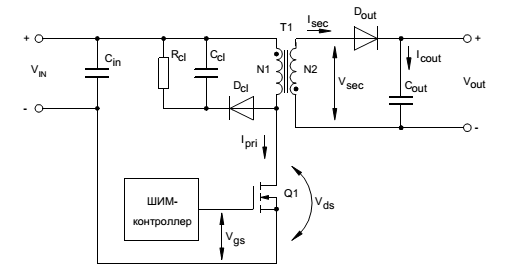
\includegraphics[width=.6\textwidth]{m_01}
    \parbox{.6\textwidth}{\caption{Силовая часть обратноходового преобразователя}\label{p01}}
\end{figure}
        На  рис.~\ref{p01} изображена силовая часть обратноходового преобразователя, а на рис.~\ref{p02}~-- диаграммы его основных токов и напряжений.
        
\begin{figure}[h!]
    \begin{minipage}{.5\textwidth}
        Будем анализировать самый распространенный режим работы~-- режим разрывных токов (\emph{discontinuous}). Это значит, что к началу  следующего цикла вся энергия из трансформатора передана в нагрузку, и следующий цикл начинаетя с нулевого тока в трансформаторе. Режим безразрывных токов (\emph{continuous}) распространен гораздо меньше.
        
        Для анализа разобьем рабочий цикл на отдельные периоды. Пусть схема работает на частоте \( f \), при этом период будет \( T = 1/f \). Интервал \( t_0 - t_1 \)~-- время включенного состояния силового ключа \( Q_1 \) (время прямого хода)~-- обозначим как \( t_{ON} \), соответственно рабочий цикл (\emph{Duty Circle}, в дальнейшем \( D \)) будет определяться как \( D = t_{ON}/T \).
        
        \textbf{Интервал \( \bm{t_0 - t_1} \).} К моменту \( t_0 \) сердечник трансформатора полностью размагничен, и ток в нем отсутствует. В момент, когда с ШИМ-контроллера подаетя управляющий сигнал, силовой
    \end{minipage} \hfill
    \begin{minipage}{.45\textwidth}
        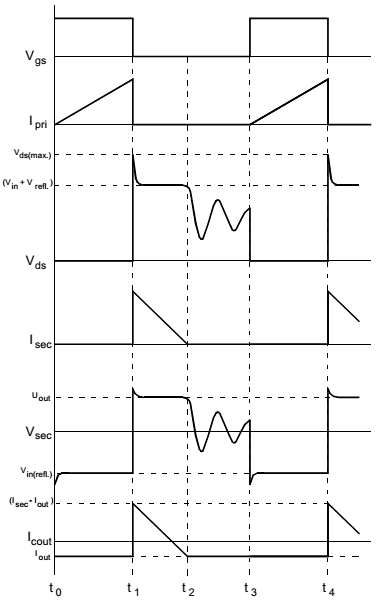
\includegraphics[width=\textwidth]{m_02}
        \parbox{\textwidth}{\caption{Диаграммы токов и напряжений обратноходового преобразователя}\label{p02}}
    \end{minipage}
\end{figure}
\noindent ключ \( Q_1 \) открывается и ток в трансформаторе начинает нарастать. То есть в идеализированной схеме включение силового транзистора происходит при нулевом токе. В реальных же условиях происходит некоторый бросок тока, связанный с зарядом паразитных емкостей трансформатора, что при больших входных напряжениях приводит к существенным потерям в ключе и возникновению паразитных высокочастотных колебаний. Для  уменьшения последних стремятся несколько замедлить процесс открывания транзистора для уменьшения паразитных токов. Выходной диод также полностью закрыт к этому времени, и нет необходимости в быстром его перезаряде/востановлении.

Ток в индуктивности первичной обмотки трансформатора \( L_{PRI} \) будет нарастать до тех пор, пока ШИМ-контроллер не даст команду на выключение силового транзистора.  ШИМ-контроллер рассчитывает (исходя из сигнала рассогласования обратной связи) количество энергии, которую необходимо запасти для поддержания постоянной мощности в нагрузке плюс потери в самом источнике. Если мощность в нагрузке обозначить как \( P_{OUT} \), то за время прямого хода мы должны запасти следующее количество энергии:
\begin{equation}
    A = \frac{P_{OUT}}{\eta\cdot f},
\end{equation}
где \( \eta \)~-- коэффициент полезного действия (КПД), а \( f \)~-- частота преобразования.

Энергия, запасаемая в индуктивности есть:
\begin{equation}
    A = \frac{L\cdot I_{PRI}^2}{2},
\end{equation}
и можно найти ток, который нарастет в первичной обмотке трансформатора за время прямого хода:
\begin{equation}
    I = \sqrt\frac{2\cdot A}{L_{PRI}} = \sqrt\frac{2\cdot P_{OUT}}{\eta\cdot f\cdot L_{PRI}}.
\end{equation}

\section{Заключение}
\newpage

\phantomsection\addcontentsline{toc}{section}{Список литературы}
\begin{thebibliography}{9}
    \bibitem{Koshljakov}Кошляков,~Н.~С. Уравнения в частных производных
    математической физики [Текст] / Кошляков~Н.~С., Глинер~Е.~Б., Смирнов~М.~М.
    Учебное пособие. -- М.: <<Высшая школа>>, 1970.-- 712с.
\end{thebibliography}
\end{document}